% Created 2021-09-11 Sat 09:35
% Intended LaTeX compiler: xelatex
\documentclass[letterpaper]{article}
\usepackage{graphicx}
\usepackage{grffile}
\usepackage{longtable}
\usepackage{wrapfig}
\usepackage{rotating}
\usepackage[normalem]{ulem}
\usepackage{amsmath}
\usepackage{textcomp}
\usepackage{amssymb}
\usepackage{capt-of}
\usepackage{hyperref}
\usepackage[margin=1in]{geometry}
\usepackage{fontspec}
\usepackage{indentfirst}
\setmainfont[ItalicFont = LiberationSans-Italic, BoldFont = LiberationSans-Bold, BoldItalicFont = LiberationSans-BoldItalic]{LiberationSans}
\newfontfamily\NHLight[ItalicFont = LiberationSansNarrow-Italic, BoldFont       = LiberationSansNarrow-Bold, BoldItalicFont = LiberationSansNarrow-BoldItalic]{LiberationSansNarrow}
\newcommand\textrmlf[1]{{\NHLight#1}}
\newcommand\textitlf[1]{{\NHLight\itshape#1}}
\let\textbflf\textrm
\newcommand\textulf[1]{{\NHLight\bfseries#1}}
\newcommand\textuitlf[1]{{\NHLight\bfseries\itshape#1}}
\usepackage{fancyhdr}
\pagestyle{fancy}
\usepackage{titlesec}
\usepackage{titling}
\makeatletter
\lhead{\textbf{\@title}}
\makeatother
\rhead{\textrmlf{Compiled} \today}
\lfoot{\theauthor\ \textbullet \ \textbf{2021-2022}}
\cfoot{}
\rfoot{\textrmlf{Page} \thepage}
\titleformat{\section} {\Large} {\textrmlf{\thesection} {|}} {0.3em} {\textbf}
\titleformat{\subsection} {\large} {\textrmlf{\thesubsection} {|}} {0.2em} {\textbf}
\titleformat{\subsubsection} {\large} {\textrmlf{\thesubsubsection} {|}} {0.1em} {\textbf}
\setlength{\parskip}{0.45em}
\renewcommand\maketitle{}
\author{Houjun Liu}
\date{\today}
\title{DNA Structures}
\hypersetup{
 pdfauthor={Houjun Liu},
 pdftitle={DNA Structures},
 pdfkeywords={},
 pdfsubject={},
 pdfcreator={Emacs 27.2 (Org mode 9.4.4)}, 
 pdflang={English}}
\begin{document}

\maketitle


\section{DNA Structures}
\label{sec:org4c60323}
\subsection{DNA double helix}
\label{sec:orge7ba9ec}
The unwrapped, raw DNA pre-bundling or formation of any structures.

\subsection{Nucleosomes}
\label{sec:org2236438}
A stack of 2 \emph{histone} groups to create a spool of 8 histone proteins
wrapping DNA

\subsection{Histones}
\label{sec:org7315eb4}
Coiler proteins that DNA wraps around to form more advanced structures

\begin{itemize}
\item Each group of histones contains 4 parts (hence 4 (per group) x 2
(groups) = 8 histones)

\begin{itemize}
\item H3, H4, H2a, H2b are the 4 wrapping proteins
\item H1 is the histone that seals the group of 4 together
\end{itemize}
\end{itemize}

\subsection{Chromatin}
\label{sec:org51fe255}
Wrapping nucleosomes into a large, fiberous structure

\subsection{Chromasome}
\label{sec:org3441cd9}
The entangling 2 chromatin together. This is the structure that is split
in half during cell replication

\begin{figure}[htbp]
\centering
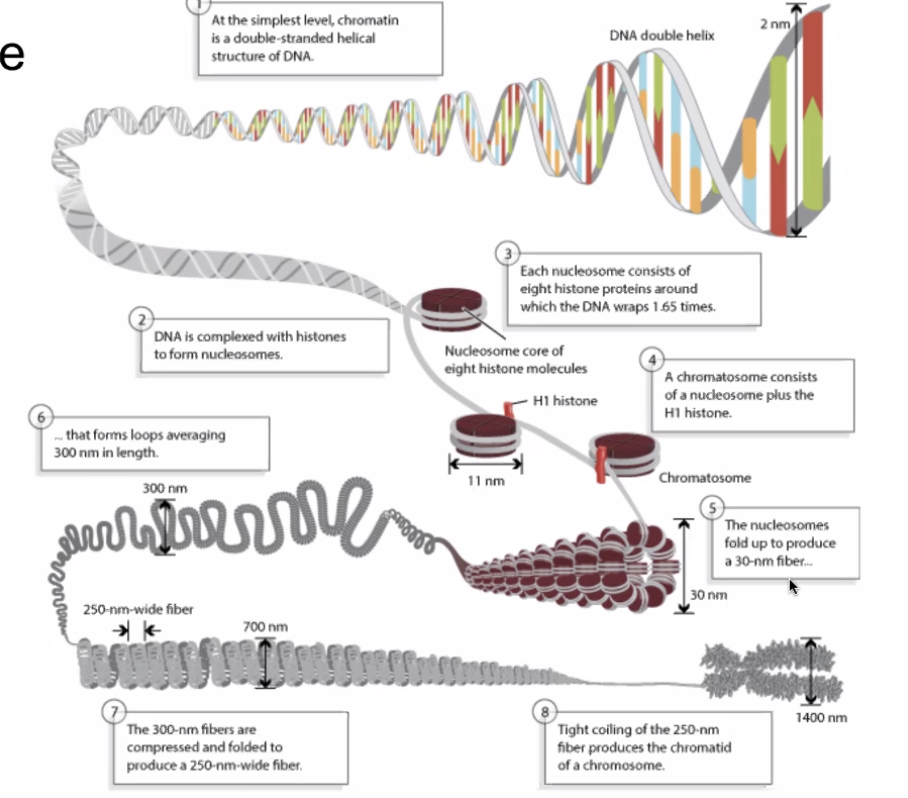
\includegraphics[width=.9\linewidth]{levelsofdna.png}
\caption{levelsofdna.png}
\end{figure}

\begin{figure}[htbp]
\centering
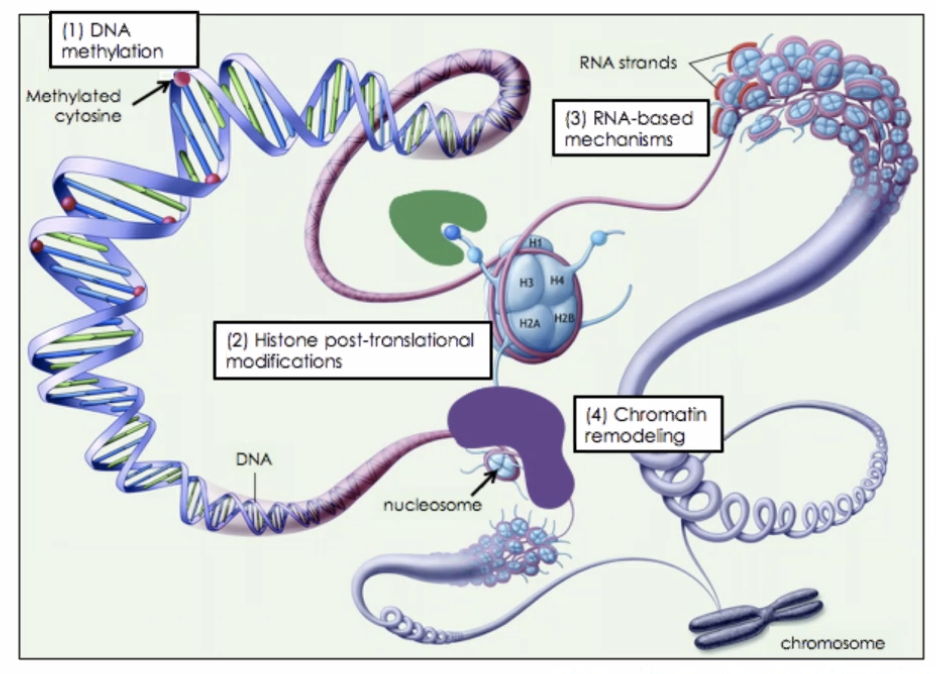
\includegraphics[width=.9\linewidth]{histones.png}
\caption{histones.png}
\end{figure}
\end{document}
